\section{Processi primari}
\label{PP}
\subsection{Descrizione}\label{PP_Descrizione}
I Processi primari comprendono tutti i processi necessari per la gestione delle funzioni principali di un progetto durante il suo ciclo di vita, in particolare permettono di individuare e di organizzare le responsabilità del fornitore verso clienti, sviluppatori, operatori, altri fornitori e manutentori del \glo{prodotto} richiesto.\\
Un progetto è in vita finché esiste un processo primario in esecuzione.
In questa sezione vengono analizzati il \textbf{processo di fornitura} e il \textbf{processo di sviluppo}.

\subsection{Processo di fornitura}
\subsubsection{Scopo del processo}\label{PF_Scopo}
Come indicato dallo \glo{standard} \glo{ISO/IEC 12207:1995} il processo di fornitura è costituito dalle \glo{attività}  svolte dal fornitore al fine di comprendere e soddisfare le richieste del proponente.\\
Il processo di fornitura è costituito dalle seguenti attività:
\begin{itemize}
	\item \textbf{Avvio:} il gruppo analizza i \glo{capitolati} proposti e redige lo \SdFv{1.0.0};
	\item \textbf{Preparazione della risposta:} il gruppo si candida con una \textit{Lettera di Presentazione} come fornitore per il \glo{capitolato} scelto;
	\item \textbf{Pianificazione:} il gruppo pianifica il lavoro da svolgere e redige i documenti previsti dal progetto;
	\item \textbf{Esecuzione e controllo:} il gruppo segue quanto pianificato e individuato dai documenti;
	\item \textbf{Revisione e valutazione:} il gruppo esegue la verifica e la validazione del prodotto;
	\item \textbf{Consegna e completamento:} il gruppo è pronto al collaudo e alla consegna del prodotto realizzato.
\end{itemize}

\subsubsection{Descrizione della sezione} 
La sezione comprende le norme principali per gestire correttamente i rapporti con il proponente \Proponente\ e i committenti \VT\ e \CR, oltre ad analizzare il documento che ha permesso al gruppo di scegliere quale progetto realizzare, ovvero lo \SdFv{1.0.0}. \\
Le norme presenti riguardano quindi:
\begin{itemize}
	\item Rapporti da mantenere con l'azienda proponente;
	\item Il materiale che il gruppo si impegna a presentare;
	\item Norme per la redazione \glo{efficace} dello \SdFv{1.0.0}.
\end{itemize}

\subsubsection{Aspettative}
Il gruppo \Gruppo\ si impegna a mantenere un rapporto costante con il proponente \Proponente\ per poter procedere nella realizzazione del progetto coerentemente a quanto richiesto e stabilito con l'azienda. 

\subsubsection{Rapporti con l'azienda proponente \Proponente}\label{Rapporti RedBabel}
Il gruppo utilizza esclusivamente i canali di comunicazione stabiliti con l'azienda proponente per le comunicazioni durante tutto il ciclo di vita del prodotto, come da accordi vengono utilizzati esclusivamente:
\begin{itemize}
	\item \glo{\textit{Slack}};
	\item \textit{Google Meet}.
\end{itemize}
Il dialogo continuo con l'azienda permette in particolare di:
\begin{itemize}
	\item Definire chiaramente i requisiti del proponente;
	\item Valutare l'andamento del lavoro;
	\item Proporre all'azienda eventuali alternative rispetto ad un determinato argomento;
	\item Chiarire eventuali dubbi emersi.
\end{itemize}

\subsubsection{Materiale fornito} 
I documenti forniti all'azienda proponente e ai committenti \VT\ e \CR\ durante la realizzazione del progetto sono:
\begin{itemize}
	\item \textbf{\textit{\AdR}:} contiene la stesura di una dettagliata specifica dei requisiti che descrive le funzionalità del prodotto richiesto comprendendo i casi d'uso individuati durante lo studio del progetto;
	\item \textbf{\textit{\PdP}:} contiene la pianificazione preventiva dei tempi e delle attività, l’analisi dei rischi e il \glo{consuntivo} di periodo, oltre alla data e ai costi previsti per la realizzazione del prodotto finale;
	\item \textbf{\textit{\PdQ}:} contiene gli obiettivi quantitativi di \glo{qualità} fissati, l'analisi degli scostamenti e le misure correttive adottate;
	\item \textbf{\textit{\Glossario}:} contiene termini utilizzati dal gruppo nella documentazione che possono creare ambiguità.
\end{itemize}
Alla documentazione è allegata la \textit{Lettera di Presentazione} con cui i membri del gruppo \Gruppo\ formalizzano il loro impegno nel portare a termine il capitolato prescelto rispettando i requisiti minimi richiesti e la data di consegna.\\
Il prodotto software finale idoneo ad accettazione viene consegnato su un supporto CD-ROM/DVD.

\subsubsection{Studio di Fattibilità}\label{SdF}
Dopo la presentazione dei capitolati d'appalto avvenuta in data 2020\_11\_05, il gruppo si riunisce per dare una prima valutazione sui vari progetti proposti e, dopo i vari seminari tecnologici, per approfondire gli aspetti positivi e negativi di ciascuno. Individuato il capitolato di interesse gli \textit{Analisti} svolgono un'ulteriore attività di analisi più approfondita e concludono la redazione dello \SdFv.\\
Il documento contiene le motivazioni che hanno spinto il gruppo a proporsi come fornitore del prodotto indicato e per ciascun capitolato riporta:
\begin{itemize}
\item Informazioni sul capitolato;
\item Descrizione del capitolato;
\item Scopo del capitolato;
\item Tecnologie coinvolte; 
\item Vincoli;
\item Aspetti positivi;
\item Aspetti critici;
\item Conclusioni.
\end{itemize}

\subsubsection{Strumenti}\label{PF_Strumenti}
Di seguito vengono riportati gli strumenti utilizzati durante il processo di fornitura.
\begin{itemize}
	\item \textbf{\textit{GanttProject}:} utilizzato per la realizzazione dei \glo{diagrammi di Gantt} all'interno del documento \PdPv{1.0.0};
	\item \textbf{\textit{Microsoft Excel}:} utilizzato per la realizzazione dei diagrammi all'interno del documento \PdPv{1.0.0}.
\end{itemize}

\newpage

\subsection{Processo di sviluppo}
\subsubsection{Scopo del processo}\label{PS_Scopo}
Lo scopo del processo di sviluppo, come stabilito dallo standard ISO/IEC 12207:1995, è descrivere i compiti e le attività da svolgere per realizzare il prodotto software richiesto.\\
In questa sezione vengono analizzate le attività per:
\begin{itemize}
	\item L'analisi dei requisiti;
	\item La progettazione del prodotto;
	\item La codifica del prodotto.
\end{itemize}

\subsubsection{Descrizione della sezione} 
Nella sezione sono trattate le attività principali del processo di sviluppo con le relative norme stabilite dal gruppo \Gruppo\ per la loro esecuzione. \\
Vengono analizzate le seguenti attività:
\begin{itemize}
\item \textbf{Analisi dei requisiti;}
\item \textbf{Progettazione architetturale;}
\item \textbf{Codifica del software.}
\end{itemize}

\subsubsection{Aspettative}
Le aspettative del gruppo riguardanti tale processo sono:
\begin{itemize}
\item Chiara individuazione dei requisiti del progetto;
\item Chiara individuazione degli obiettivi del progetto;
\item Chiara individuazione dei rischi del progetto;
\item Chiara individuazione dei vincoli di design;
\item Codifica del software coerente con i requisiti del proponente che supera i \glo{test} di qualità previsti.
\end{itemize}

\subsubsection{Analisi dei requisiti}
\myparagraph{Scopo dell'attività} 
L'attività di analisi dei requisti viene svolta dagli \textit{Analisti} incaricati per individuare i requisiti che il prodotto deve soddisfare.
I requisiti possono essere esplicitamente richiesti dal proponente o individuati implicitamente tramite l'attività di analisi, possono essere individuati direttamente o indirettamente perché dipendono da altri requisiti.\\
L'individuazione dei requisiti consente di:
\begin{itemize}
	\item Realizzare un prodotto software che soddisfi i bisogni del proponente;
	\item Facilitare le revisioni del codice;
	\item Fornire delle linee guida per le attività di test.
\end{itemize}

\myparagraph{Descrizione della sezione}
La sezione contiene le norme relative all'attività di analisi dei requisiti e del relativo documento \AdR\ che i componenti del gruppo, in particolare gli \textit{Analisti}, devono seguire.

\myparagraph{Aspettative}\label{AspettativeAnalisi}L'attività di analisi dei requisiti ha come obiettivo la redazione del documento di \AdR{} che comprende in modo formale tutti i requisiti che il prodotto software deve o è desiderabile soddisfi. Per assicurare il raggiungimento degli obiettivi di qualità previsti dal \PdQ\ il gruppo intende:
\begin{itemize}
	\item Coinvolgere frequentemente proponente e committente;
	\item Studiare prodotti simili a quello richiesto;
	\item Valutare i possibili scenari immedesimandosi nell'utente del prodotto;
	\item Individuare requisiti che possono migliorare la qualità del prodotto anche se non obbligatori;
	\item Assicurare che l'implementazione del prodotto soddisfi i requisiti individuati in modo coerente rispetto al loro significato.
\end{itemize}

\myparagraph{Struttura del documento}
La struttura del documento comprenderà:
\begin{itemize}
	\item \textbf{Descrizione:} definisce le caratteristiche, i vincoli e gli obiettivi del prodotto;
	\item \textbf{Casi d'uso:} contiene tutte le informazioni utili per descrivere gli scenari che l'utente del prodotto può incontrare, comprendendo anche la loro rappresentazione attraverso i diagrammi UML;
	\item \textbf{Requisiti:} viene inserita una tabella contenente:
	\begin{itemize}
		\item Codice identificativo del requisito;
		\item Descrizione del requisito;
		\item Fonte dalla quale è stato individuato il requisito. 
	\end{itemize} 
\end{itemize}

\myparagraph{Classificazione dei requisiti}\label{ClassificazioneRequisiti}Tutti i requisti sono individuati da un codice identificativo univoco rappresentato nel seguente modo:

\begin{center}
	\textbf{R[Tipologia][Rilevanza][Numero][\_Codice]}
\end{center}

\begin{itemize}
	\item \textbf{Tipologia:} rappresenta il tipo di requisito, può assumere i seguenti valori:
	\begin{itemize}
		\item \textbf{V:} requisito di \textbf{vincolo};
		\item \textbf{F:} requisito \textbf{funzionale};
		\item \textbf{P:} requisito \textbf{prestazionale};
		\item \textbf{Q:} requisito di \textbf{qualità}.
	\end{itemize}
	\item \textbf{Rilevanza:} rappresenta l'utilità del requisito che va negoziata e concordata con il committente, può assumere i seguenti valori:
	\begin{itemize}
		\item \textbf{O:} requisito \textbf{obbligatorio}, deve essere soddisfatto perché irrinunciabile per qualcuno degli \glo{stakeholder};
		\item \textbf{D:} requisito \textbf{desiderabile}, non strettamente necessario ma aumenta la completezza del prodotto. Questi requisiti vengono negoziati con l'azienda \Proponente;
		\item \textbf{Z:} requisito \textbf{opzionale}, relativamente utile anch'esso ed è contrattabile con l'azienda \Proponente.
	\end{itemize}
	\item \textbf{Numero:} numero progressivo che parte da 1.
	\item \textbf{Codice:} opzionale, identifica il caso d'uso generico e gli eventuali sotto-casi ad esso associati, è rappresentato da:
	\begin{center}
		\textbf{[NumeroCasoBase](.NumeroSottoCaso)*}
	\end{center}
	dove NumeroCasoBase e NumeroSottoCaso sono rappresentati da numeri progressivi.\\
	I sotto-casi possono ramificarsi ulteriormente portandoli ad avere a loro volta altri sotto-casi.
\end{itemize}

\begin{table}[h]
	\centering
	\caption{Esempio di classificazione requisito} 
	
\rowcolors{2}{white}{celeste} 
\renewcommand{\arraystretch}{1.5}
\begin{tabular}{|c c c|} 
	
	\rowcolor{darkblue}
	\textcolor{white}{\textbf{Codice Requisito}}&
	\textcolor{white}{\textbf{Descrizione}}&
	\textcolor{white}{\textbf{Fonte}}\\	

	RFO1\_1.1 & ......... & Capitolato\\
	\hline
\end{tabular}
\end{table}

\myparagraph{Requisiti di processo}\label{RequisitiProcesso}Dopo un confronto con il \VT\ si è ritenuto opportuno riportare i requisiti presenti nell'\AdR\ ritenuti da noi requisiti di processo all'interno di questo documento.\\
\begin{table}[h]
	\centering
	\caption{Requisiti di processo} 
\rowcolors{2}{white}{celeste} 
\renewcommand{\arraystretch}{1.5}
\begin{tabular}{|C{9.5cm} C{2.5cm}|} 
	
	\rowcolor{darkblue}
	\textcolor{white}{\textbf{Descrizione}}&
	\textcolor{white}{\textbf{Fonte}}\\	

	La piattaforma deve essere sviluppata \glo{production-ready}. & Capitolato\\
	Il codice sorgente deve essere realizzato con un sistema di \glo{versionamento} e caricato in una \glo{repository} su \glo{GitHub}. & Capitolato\\
	Il codice sorgente deve essere sottoposto ad analisi statica attraverso lo strumento \glo{Typescript-eslint}. & Capitolato\\
	Devono essere realizzati test di integrazione per verificare l’integrazione con i sottosistemi. & Capitolato\\
	Devono essere realizzati test d’unità per verificare le singole componenti del prodotto. & Interna\\
	\hline
\end{tabular}
\end{table}

\myparagraph{Classificazione dei casi d'uso}
Tutti i casi d'uso analizzati sono individuati da un codice identificativo univoco rappresentato nel seguente modo:

\begin{center}
	\textbf{UC[NumeroCasoBase](.NumeroSottoCaso)*}
\end{center}
dove:
\begin{itemize}
	\item \textbf{NumeroCasoBase:} è costituito da un numero progressivo che indica il caso d'uso generico;
	\item \textbf{NumeroSottoCaso} è costituito da un numero progressivo opzionale che indica il sotto-caso d'uso del caso d'uso generico.
\end{itemize}  
I sotto-casi possono avere a loro volta altri sotto-casi.\\ 
I casi d'uso analizzati comprenderanno:
\begin{itemize}
	\item \textbf{Codice identificativo:} assegnato secondo quanto stabilito precedentemente;
	\item \textbf{Nome:} titolo assegnato al caso d'uso e indicato dopo il codice identificativo;
	\item \textbf{Rappresentazione grafica:} descrizione grafica del caso d'uso attraverso lo standard \glo{UML};
	\item \textbf{Descrizione:} breve descrizione testuale del caso d'uso;
	\item \textbf{Attori:} rappresentano gli utenti che hanno un'interazione con il sistema, si dividono in:
	\begin{itemize}
		\item \textbf{Attori primari:} svolgono attivamente il caso d'uso;
		\item \textbf{Attori secondari:} sono entità estranee al sistema che supportano gli attori primari nelle loro attività.
	\end{itemize}
	\item \glo{\textbf{Precondizioni:}} condizioni del sistema prima degli eventi che determinano il caso d'uso;
	\item \glo{\textbf{Postcondizioni:}} condizioni del sistema dopo il verificarsi degli eventi che hanno determinato il caso d'uso;
	\item \textbf{Trigger:} opzionale, evento scatenante del caso d'uso;
	\item \textbf{Scenario principale:} elenco del flusso di eventi del caso d'uso;
	\item \textbf{Scenario alternativo:} opzionale, elenco delle azioni che si verificano allo scatenarsi di un evento non previsto rispetto allo scenario principale del caso d'uso;
	\item \textbf{Inclusioni:} opzionali, si ha inclusione quando un caso d'uso è incondizionatamente incluso nell'esecuzione del caso d'uso in esame;
	\item \textbf{Estensioni:} opzionali, si ha estensione quando l'esecuzione di un caso d'uso interrompe l'esecuzione del caso d'uso in esame;
	\item \textbf{Generalizzazioni:} opzionali, si ha generalizzazione quando si intende aggiungere o modificare caratteristiche base di un caso d'uso a un altro caso d'uso.
\end{itemize}

\myparagraph{Qualità dell'analisi dei requisiti}\label{QualitàAnalisi}Come indicato dallo standard IEEE 830-1998, la specifica deve essere:
\begin{itemize}
	\item \textbf{Priva di ambiguità:} i requisiti devono rispettare chiaramente i bisogni dell'utente finale del prodotto;
	\item \textbf{Corretta:} i requisiti devono essere coerenti rispetto alle richieste degli utenti finali;
	\item \textbf{Completa:} i requisiti presenti permettono la completa comprensione del dominio del problema;
	\item \textbf{Verificabile:} deve essere possibile verificare il soddisfacimento dei requisiti da parte del prodotto;
	\item \textbf{Consistente:} i requisiti non devono essere contraddittori tra loro;
	\item \textbf{Modificabile:} i requisiti devono poter essere modificati senza perdita di consistenza e completezza;
	\item \textbf{Tracciabile:} l'origine dei requisiti è chiara e facilmente rintracciabile;
	\item \textbf{Ordinata per rilevanza:} i requisiti devono essere classificati secondo la loro rilevanza rispetto a quanto contrattato con il proponente.
\end{itemize}

\myparagraph{Metriche}\label{MAnalisi}Di seguito vengono presentate le metriche utilizzate per garantire il controllo sulla qualità. Per una descrizione sullo standard di riferimento e un elenco completo di tutte le metriche applicate si rimanda alla sezione \S\ref{9126} dell'appendice.
\begin{itemize}
\item\textbf{MPR01: Soddisfacimento requisiti obbligatori}\hypertarget{MSoddRequisiti}\\
Indica la percentuale di requisiti obbligatori soddisfatti nel momento in cui viene calcolato.\\
Viene calcolato nel seguente modo:
	\begin{center}
		\textbf{RO=\(\frac{ROC}{RO}\)*100}
	\end{center}
	dove:
	\begin{itemize}
		\item \textbf{RO} sta per \textbf{requisiti obbligatori};
		\item \textbf{ROC} sta per \textbf{requisiti obbligatori coperti dall'implementazione}.
	\end{itemize}
\end{itemize}
\subsubsection{Progettazione}
\myparagraph{Scopo dell'attività} \label{PS_Progettazione_Scopo}
La progettazione ha lo scopo di definire quale sarà l'architettura logica del prodotto, viene svolta dai \textit{Progettisti} prima dell'attività di codifica. Una buona architettura consente di:
\begin{itemize}
	\item Ridurre la complessità del prodotto al fine di facilitare l'attività di codifica;
	\item Organizzare e ripartire le responsabilità di realizzazione;
	\item Realizzare un prodotto garantendo qualità e utilizzando il minor numero di risorse.
\end{itemize} 

\myparagraph{Descrizione della sezione}
La sezione contiene le norme relative all'attività di progettazione che i componenti del gruppo, in particolare i \textit{Progettisti}, devono seguire.

\myparagraph{Aspettative}
Il gruppo per questa attività si aspetta di definire l'architettura logica del prodotto rispettandone le caratteristiche di qualità.

\myparagraph{Qualità dell'attività di progettazione}\label{QualitàProgettazione}
Un'architettura di buona qualità ha come caratteristiche misurabili e osservabili oggettivamente:
\begin{itemize}
	\item \textbf{Sufficienza:} capace di soddisfare tutti i requisiti indicati nell'\AdRv;
	\item \textbf{Comprensibilità:} capace di essere capita da tutti gli stakeholders;
	\item \textbf{Modularità:} suddivisa in parti chiare e ben distinte;
	\item \textbf{Robustezza:} capace di gestire eventi non previsti causati dall'utente e dall'ambiente;
	\item \textbf{Flessibilità:} permette modifiche a costo contenuto al variare dei requisti;
	\item \textbf{Riusabilità:} le sue parti possono essere utilizzate in altre applicazioni;
	\item \textbf{Affidabilità:} svolge quanto previsto;
	\item \textbf{Sicura:} capace di resistere a malfunzionamenti ed evitare possibili intrusioni.
\end{itemize}
Le sue componenti devono essere semplici, coese nel raggiungimento degli obiettivi, incapsulate e con un basso livello di accoppiamento.
I \textit{Progettisti} devono assicurare che l'architettura e le sue componenti presentino le caratteristiche descritte e superino dei test di qualità da loro definiti.

\myparagraph{Periodi della progettazione}\label{PeriodiProgettazione}
L'attività di progettazione si articola in due parti: 
\paragraph*{Progettazione Architetturale} 
Vengono definite le specifiche dell'architettura e delle componenti del prodotto, delle loro interazioni con le restanti parti del sistema e dei \glo{test di integrazione}. Al termine di questo periodo di progettazione si ottiene la \glo{\textit{Technology Baseline}} del progetto che conterrà: 
\begin{itemize}
	\item \glo{\textbf{Proof of Concept:}} primo eseguibile del sistema in grado di dimostrare che la tecnologia selezionata serve in modo efficace allo sviluppo del prodotto atteso;
	\item \textbf{Tecnologie utilizzate:} descrizione dettagliata delle tecnologie impiegate nello sviluppo del progetto, con particolare enfasi sui pregi e i difetti riscontrati;
	\item \textbf{Test di integrazione:} definizione dei test eseguiti per verificare che le varie componenti del sistema, una volta integrate insieme, interagiscano in modo corretto e in conformità con quanto richiesto dai requisiti;
	\item \textbf{Tracciamento delle componenti:} associazione tra requisiti e componenti che li soddisfano.
\end{itemize}

\paragraph*{Progettazione di dettaglio}
Vengono definite le specifiche di dettaglio dell'architettura suddividendo il sistema fino ad arrivare a singole unità ben definite e realizzabili da un singolo programmatore. Al termine di questo periodo di progettazione si ottiene la \textit{\glo{Product Baseline}} del progetto che conterrà: 
\begin{itemize}
	\item \glo{\textbf{Design Pattern:}} descrizione dei design pattern utilizzati nella definizione dell'architettura, per la soluzione progettuale a problemi ricorrenti riscontrati; ogni design pattern deve essere opportunamente descritto, con una spiegazione del suo significato, ed accompagnato da un diagramma che ne mostri la struttura;
	\item \textbf{Diagrammi UML:} diagrammi realizzati in linguaggio \textit{UML} versione 2.0, utilizzati per rendere più chiare le soluzioni progettuali adottate; 
	\item \glo{\textbf{Test di unità:}} definizione dei test eseguiti per verificare che il funzionamento delle varie classi e metodi che implementano il sistema software sia corretto e conforme ai requisiti;
	\item \textbf{Tracciamento delle classi:} associazione tra requisiti e classi che li soddisfano.
\end{itemize}

\myparagraph{Diagrammi UML 2.0}\label{DiagrammiUML}
I diagrammi UML sono diagrammi realizzati in linguaggio \textit{UML}, utilizzati per chiarire le scelte progettuali adottate e ridurre eventuali ambiguità. 
Di seguito vengono analizzati i diagrammi utilizzati.
\paragraph*{Diagrammi delle classi}
Questi diagrammi descrivono il tipo degli oggetti che fanno parte di un sistema.\\
Gli elementi di un diagramma di classe sono:
\begin{itemize}
	\item \textbf{Nome:} nome della classe scritto in inglese a lettere maiuscole e in grassetto. Nel caso di classe \textit{astratta} il nome deve essere in formato italico, nel caso di un'\textit{interfaccia} deve essere preceduto dalla direttiva \textbf{$\ll$interface$\gg$};
	\item \textbf{Attributi:} la definizione di un attributo segue il formato:
	\begin{center}
		\textbf{Visibilità nome: tipo [molteplicità] = default [proprietà aggiuntive]}
	\end{center}
	\begin{itemize}
		\item \textbf{Visibilità:} visibilità dell'attributo rispetto ad altre classi, può essere:
		\begin{itemize}
			\item -: visibilità privata;
			\item +: visibilità pubblica;
			\item \#: visibilità protetta;
			\item $\sim$: visibilità di package.
		\end{itemize}
		\item \textbf{Nome:} nome dell'attributo, se l'attributo è \textit{costante} il nome deve essere scritto in maiuscolo, se di tipo \textit{statico} il nome va sottolineato;
		\item \textbf{Tipo:} tipo di dato dell'attributo;
		\item \textbf{Molteplicità:} occorrenze dell'attributo nella classe, il campo è opzionale;
		\item \textbf{Valore di default:} valore predefinito dell'attributo;
		\item \textbf{Proprietà aggiuntive:} eventuali proprietà ritenute importanti, il campo è opzionale.
	\end{itemize}
	\item \textbf{Operazioni:} rappresentano le azioni eseguibili dalla classe, la definizione di una operazione segue il formato:
	\begin{center}
		\textbf{Visibilità nome [lista-parametri] : tipo-ritorno [proprietà aggiuntive]}
	\end{center}
	\begin{itemize}
		\item \textbf{Visibilità:} visibilità dell'operazione rispetto ad altre classi indicata come per gli attributi;
		\item \textbf{Nome:} nome dell'operazione, se l'operazione è \textit{astratta} il nome deve essere scritto in italico, se di tipo \textit{statico} il nome va sottolineato;
		\item \textbf{Lista-parametri:} lista dei parametri dell'operazione; 
		\item \textbf{Return-type:} tipo di ritorno dell'operazione;
		\item \textbf{Proprietà aggiuntive:} eventuali proprietà ritenute importanti, il campo è opzionale.
	\end{itemize}
\end{itemize}
I diagrammi delle classi sono collegati tra loro tramite \textbf{relazioni di dipendenza}, la modifica di un elemento di un diagramma può cambiarne la definizione di un altro.
Le relazioni di dipendenza previste sono:
	\begin{itemize}
		\item \textbf{Dipendenza:} gli oggetti di una classe A utilizzano brevemente gli oggetti di un'altra classe B, l'associazione esiste per un tempo limitato;
		\begin{center}
			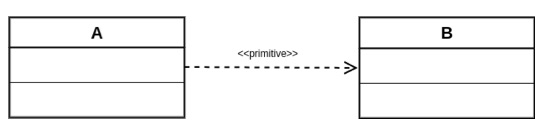
\includegraphics[scale=0.4]{Immagini/UML/Dipendenza} \\
			\captionof{figure}{Dipendenza fra classi}
		\end{center}
		\item \textbf{Associazione:} la classe A contiene dei campi dati o delle istanze di un'altra classe B. Le molteplicità possibili sono:
		\begin{itemize}
			\item \textbf{1:} A possiede un'istanza di B;
			\item \textbf{0..1:} A possiede 0 o 1 istanze di B;
			\item \textbf{0..*:} A possiede 0 o più istanze di B;
			\item \textbf{*:} A possiede più istanze di B.
		\end{itemize}
		\begin{center}
			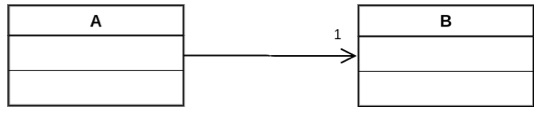
\includegraphics[scale=0.4]{Immagini/UML/Associazione} \\
			\captionof{figure}{Associazione fra classi}
		\end{center}
		\item \textbf{Aggregazione:} la classe A possiede un riferimento ad un oggetto di un'altra classe B che può essere condiviso, l'aggregato B non ha senso di esistere senza l'aggregante A;
		\begin{center}
			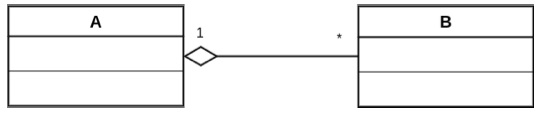
\includegraphics[scale=0.4]{Immagini/UML/Aggregazione}\\
			\captionof{figure}{Aggregazione fra classi}
		\end{center}
		\item \textbf{Composizione:} la classe A possiede un oggetto di un'altra classe B, solo l'oggetto intero può creare e distruggere le sue parti;
		\begin{center}
			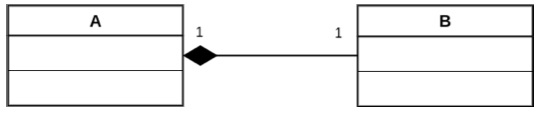
\includegraphics[scale=0.4]{Immagini/UML/Composizione} \\
			\captionof{figure}{Composizione fra classi}
		\end{center}
		\item \textbf{Generalizzazione:} la classe A generalizza un'altra classe B se ogni oggetto di B è anche un oggetto di A;
		\item \textbf{Subtyping:}  la classe A implementa l'interfaccia B. 
		\begin{center}
				\begin{minipage}{0.4\textwidth}
					\begin{center}
						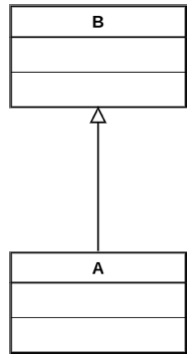
\includegraphics[scale=0.4]{Immagini/UML/Generalizzazione}\\
						\captionof{figure}{Generalizzazione fra classi}
					\end{center}
			\end{minipage}
			\begin{minipage}{0.5\textwidth}
				\begin{center}
						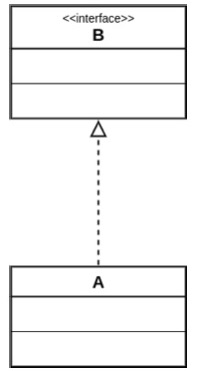
\includegraphics[scale=0.385]{Immagini/UML/Subtyping}\\
					\captionof{figure}{Subtyping fra classi}
				\end{center}
			\end{minipage}
		\end{center}	
	\end{itemize}

\paragraph*{Diagrammi dei package}
Un package rappresenta un raggruppamento di un numero arbitrario di elementi \textit{UML} in una unità di livello più alto, può quindi contenere classi (anche astratte), un altro package e interfacce. Ogni elemento di un package, identificativo di un \glo{namespace}, può avere visibilità pubblica(+) o privata(-) e deve avere un nome completamente qualificato secondo lo schema: 
\begin{center}
	\textbf{package::package::...::classe}
\end{center}
I diagrammi dei package documentano le dipendenze tra le classi che dovrebbero seguire tutte la stessa direzione evitando le dipendenze circolari.

\paragraph*{Diagrammi delle attività}
Questi diagrammi descrivono la logica procedurale e i processi di business, aiutando a descrivere gli aspetti dinamici dei casi d'uso. \\
Gli elementi di un diagramma di attività sono:
\begin{itemize}
	\item \textbf{Token:} vengono prodotti e consumati durante l'esecuzione;
	\item \textbf{Nodo iniziale:} rappresenta il punto d'inizio dell'esecuzione dell'attività, genera token;
	\item \textbf{Nodo di fine flusso:} rappresenta un punto di terminazione di un percorso di esecuzione, l'attività può continuare su altri percorsi;
	\item \textbf{Nodo finale:} rappresenta il punto di terminazione dell'esecuzione dell'attività, consuma token;
	\begin{center}
		\begin{minipage}{0.3\textwidth}
			\centering
			
\includegraphics[scale=0.2]{Immagini/UML/NodoIniziale}
			\captionof{figure}{Nodo iniziale}
		\end{minipage}
		\begin{minipage}{0.3\textwidth}
			\centering
			
\includegraphics[scale=0.2]{Immagini/UML/NodoFineFlusso}
			\captionof{figure}{Nodo fine flusso}
		\end{minipage}
		\begin{minipage}{0.3\textwidth}
			\centering
			
\includegraphics[scale=0.19]{Immagini/UML/NodoFinale}
			\captionof{figure}{Nodo finale}
		\end{minipage}
	\end{center}
	\item \textbf{Activity:} rappresenta un'azione all'interno dell'attività, identificata da una breve descrizione;
	\item \textbf{Subactivity:} rappresenta una sotto-attività utilizzata per descrivere un'azione che ne comprende altre al suo interno, il suo diagramma viene fornito separatamente. Ogni sotto-attività è composta dall'input, dall'output e dalle azioni contenute.
	\begin{center}
		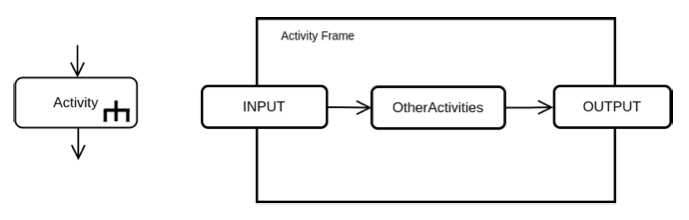
\includegraphics[scale=0.4]{Immagini/UML/Sottoattivita}
		\captionof{figure}{Attività che presenta una sotto-attività}
	\end{center}
	\item \textbf{Pin:} rappresenta un parametro prodotto o consumato da un'azione, va indicato il formato del parametro;
	\begin{center}
		\centering
		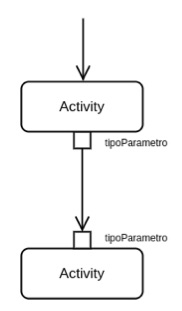
\includegraphics[scale=0.4]{Immagini/UML/Pin}
		\captionof{figure}{Attività che presenta un pin}
	\end{center}
	\item \textbf{Fork:} rappresenta un punto d'inizio di un elaborazione parallela all'interno dell'attività, produce un token per ogni processo;
	\item \textbf{Join:} rappresenta un punto di sincronizzazione tra i processi paralleli, consuma i token in ingresso e ne genera solo uno;
	\item \textbf{Branch:} rappresenta un punto di decisione tra i possibili percorsi di esecuzione in base alla guardia associata;
	\item \textbf{Merge:} rappresenta un punto di unione dei diversi percorsi di esecuzione (non paralleli) generati in seguito ad un branch, il token viene solo instradato;
	\begin{center}
		\begin{minipage}{0.4\textwidth}
			\centering
			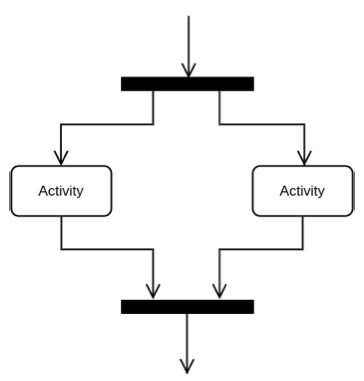
\includegraphics[scale=0.453]{Immagini/UML/ForkJoin}
			\captionof{figure}{Fork e Join}
		\end{minipage}
		\begin{minipage}{0.4\textwidth}
			\centering
			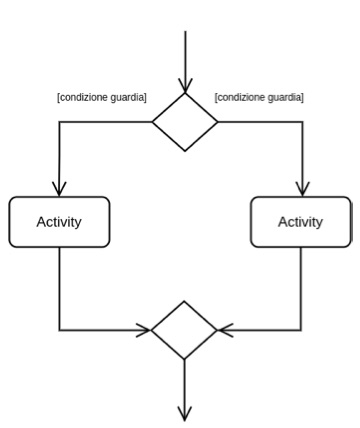
\includegraphics[scale=0.4]{Immagini/UML/BranchMerge}
			\captionof{figure}{Branch e Merge}
		\end{minipage}
	\end{center}
	\item \textbf{Segnale:} rappresenta un evento esterno, generato in modo non bloccante e catturato in modo bloccante, all'interno dell'attività;
	\begin{center}
		\centering
		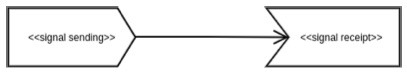
\includegraphics[scale=0.5]{Immagini/UML/Segnali}
		\captionof{figure}{Segnali in un diagramma attività}
	\end{center}
	\item \textbf{Timeout:} rappresenta un'attesa bloccante all'interno dell'attività, di cui deve essere specificata la durata e l'unità di misura, o un evento ripetuto nel tempo;
	\begin{center}
		\centering
		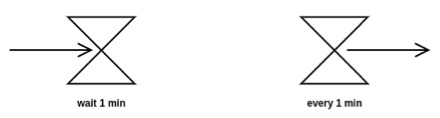
\includegraphics[scale=0.5]{Immagini/UML/Timeout}
		\captionof{figure}{Timeout in un diagramma attività}
\end{center}
	\item \textbf{Swimlane:} fornisce una responsabilità all'esecuzione delle azioni all'interno di un'attività.
\end{itemize}

\paragraph*{Diagrammi di sequenza}
I diagrammi di sequenza descrivono la collaborazione di un gruppo di oggetti che devono implementare collettivamente un comportamento.
Gli elementi utilizzati in questi diagrammi sono i seguenti:
\begin{itemize}
	\item \textbf{Partecipante:} entità che detiene il flusso di esecuzione del caso d'uso, è composto di due parti:
	\begin{itemize}
		\item \textbf{Nome:} nome dell'entità partecipante;
		\item \textbf{Barra di attivazione:} indica il periodo di tempo durante il quale il partecipante è attivo;
	\end{itemize}
	\item \textbf{Messaggio:} rappresenta dati e operazioni scambiati tra partecipanti, può essere di una delle seguenti tipologie:
	\begin{itemize}
		\item \textbf{Sincrono:} il chiamante rimane in attesa della risposta;
		\item \glo{\textbf{Asincrono:}} il chiamante non attende la risposta; 
		\item \textbf{Ritorno:} messaggio di ritorno riferito ad un precedente messaggio di chiamata;
		\item \textbf{Creazione:} messaggio di creazione di un nuovo partecipante da parte del partecipante chiamante;
		\item \textbf{Distruzione:} messaggio di distruzione di un partecipante da parte del partecipante chiamante.
	\end{itemize}
\end{itemize}
\begin{center}
	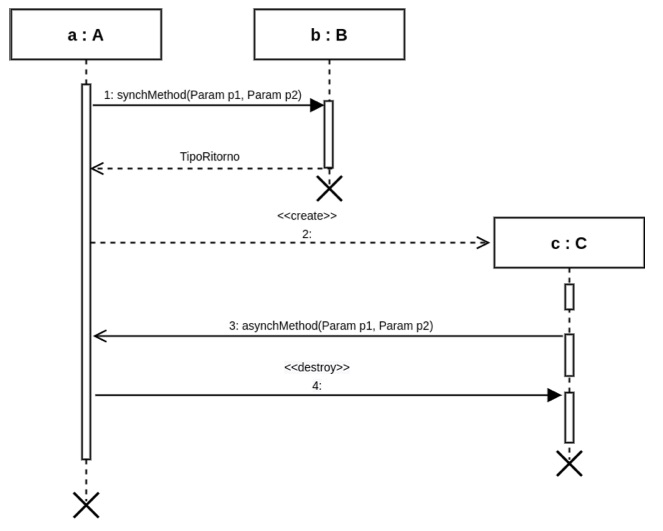
\includegraphics[scale=0.5]{Immagini/UML/DSequenza} \\
	\captionof{figure}{Esempio di diagramma di sequenza}
\end{center}

\paragraph*{Diagrammi dei casi d'uso}
Un caso d'uso è un'insieme di scenari (sequenze di azioni) che hanno in comune uno scopo finale per un utente. I diagrammi dei casi d'uso sono una rappresentazione grafica dei casi d'uso analizzati nel documento di \AdRv. Vengono messi in evidenza:
\begin{itemize}
	\item \textbf{Attori:} rappresentano tutto ciò che è esterno al sistema e interagisce con esso;
	\item \textbf{Use Case:} rappresentano le attività associate al sistema.
\end{itemize}
Le eventuali relazioni tra gli Use Case del sistema rappresentate in questi diagrammi sono: 
\begin{itemize}
	\item \textbf{Inclusione:} si ha quando vi sono funzionalità comuni fra più casi d'uso, lo use case B è incondizionatamente incluso nell'esecuzione dello use case A;
	\begin{center}
		\centering
		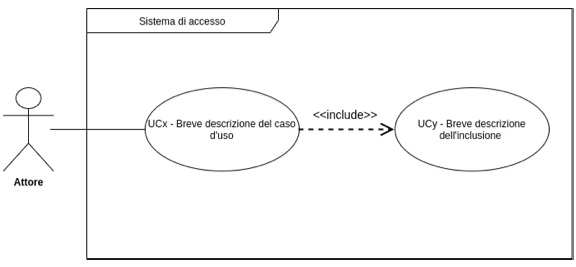
\includegraphics[scale=0.4]{Immagini/UML/Inclusione}
		\captionof{figure}{Inclusione casi d'uso}
	\end{center}
	\item \textbf{Estensione:} si ha se ogni istanza dello use case A esegue lo use case B in modo condizionato, l'esecuzione di B interrompe A;
	\begin{center}
		\centering
		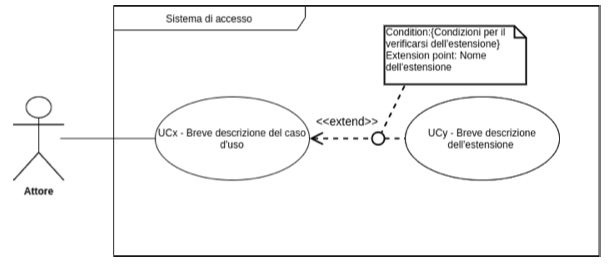
\includegraphics[scale=0.4]{Immagini/UML/Estensione}
		\captionof{figure}{Estensione casi d'uso}
	\end{center}
	\item \textbf{Generalizzazione:} si ha quando si vogliono aggiungere o modificare caratteristiche base, in particolare si ha che:
	\begin{itemize}
		\item L'attore A è generalizzazione dell'attore B se B condivide almeno le funzionalità di A;
		\item I casi d'uso figli aggiungono funzionalità rispetto ai padri o ne modificano il comportamento.
	\end{itemize}
	\begin{center}
		\begin{minipage}{0.4\textwidth}
			\centering
			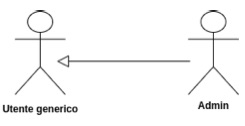
\includegraphics[scale=0.4]{Immagini/UML/GeneralizzazioneAttori}
			\captionof{figure}{Generalizzazione tra attori}
		\end{minipage}
		\begin{minipage}{0.5\textwidth}
			\centering
			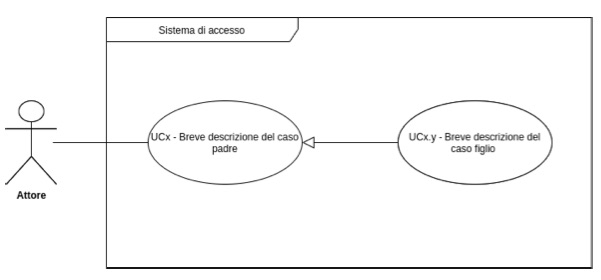
\includegraphics[scale=0.4]{Immagini/UML/GeneralizzazioneUC}
			\captionof{figure}{Generalizzazione Casi d'uso}
	\end{minipage}
	\end{center}
\end{itemize} 




\subsubsection{Codifica software}
\myparagraph{Scopo dell'attività} 
L'attività di codifica svolta dai \textit{Programmatori} ha lo scopo di trasformare in codice quanto previsto dall'attività di progettazione svolta dai \textit{Progettisti}, procedendo all'effettiva realizzazione del prodotto software richiesto.

\myparagraph{Descrizione della sezione}
La sezione tratta le norme da seguire per ogni linguaggio di programmazione utilizzato durante lo svolgimento del progetto.

\myparagraph{Aspettative}\label{AspettativeCodifica}Con le norme individuate il gruppo si aspetta la realizzazione di codice uniforme. Per assicurare il raggiungimento degli obiettivi di qualità previsti dal \PdQ\ il gruppo intende:
\begin{itemize}
	\item Utilizzare i linguaggi sfruttando adeguatamente le loro capacità;
	\item Ridurre il numero di righe di codice che possono causare errori;
	\item Redarre il codice affinché si chiaro nel tempo e facilmente comprensibile anche da altri programmatori.
\end{itemize}

\myparagraph{Qualità della codifica}
La codifica è di qualità se: 
\begin{itemize}
	\item Il codice è facilmente leggibile;
	\item I costrutti del linguaggio sono utilizzati in modo chiaro e coerente;
	\item La compilazione non presenta errori fatali o potenziali.
\end{itemize}
Queste caratteristiche sono in grado di agevolare manutenzione, verifica e validazione e di conseguenza migliorare la qualità di prodotto.

\myparagraph{Convenzioni generiche}\label{CodificaConvenzioni}
Vengono di seguito riportate le norme generiche stabilite per la codifica.
\paragraph*{Intestazione}
I file sorgenti consegnati presentano la seguente intestazione inserita in un blocco di commento.
\paragraph*{Nomenclatura}
Tutte le classi, i metodi, le variabili devono avere un nome univoco, esplicativo e scritto in lingua inglese, in particolare:
\begin{itemize}
	\item Per i nomi di cartelle, file e classi viene seguita la convenzione \textbf{CamelCase};
	\item I nomi di variabili e metodi hanno iniziale minuscola, se composti da più parole la prima lettera delle parole successive alla prima è maiuscola;
	\item Le costanti vengono scritte in maiuscolo.
\end{itemize}
\paragraph*{Parentesi}
I blocchi di codice vanno inseriti tra parentesi graffe, anche se il blocco è vuoto o costituito da una sola riga di codice.
\paragraph*{Verbosità}
Una riga di codice deve essere lunga al massimo 140 caratteri. Se possibile è desiderabile definire metodi brevi evitando la ricorsione.

\myparagraph{Metriche}\label{MCodifica}Di seguito vengono presentate le metriche utilizzate per garantire il controllo sulla qualità. Per una descrizione sullo standard di riferimento e un elenco completo di tutte le metriche applicate si rimanda alla sezione \S\ref{9126} dell'appendice. 
\begin{itemize}
	\item\textbf{MPDS01: Completezza dell'implementazione}\hypertarget{MCImplementazione} \\
	L'indice stabilisce la completezza del prodotto software realizzato nel momento in cui viene calcolato rispetto a tutti i requisiti previsti dall'\AdRv{1.0.0}.\\
	Viene calcolato nel seguente modo:
	\begin{center}
		\textbf{CI=\(1-\frac{FNI}{FI}\)*100}
	\end{center}
	dove:
	\begin{itemize}
		\item \textbf{FNI} indica il numero di funzionalità non implementate;
		\item \textbf{FI} indica il numero di funzionalità implementate.
	\end{itemize}
\item\textbf{MPDS02: Densità errori} \hypertarget{MErrori}\\
Rappresenta la percentuale di righe di codice che possono causare errori.\\
Viene calcolato nel seguente modo:
\begin{center}
	\textbf{DE=\(\frac{RB}{RTOT}\)*100}
\end{center}
dove:
\begin{itemize}
	\item \textbf{RB} indica il numero di linee di codice che possono causare imprevisti o comportamenti diversi da quelli desiderati;
	\item \textbf{RTOT} indica il numero di linee di codice totali.
\end{itemize}

\item\textbf{MPDS07: Facilità di comprensione} \hypertarget{MFComprensione}\\
Il valore indica la facilità di comprensione del codice in base al numero di righe di commento presenti.\\
Viene calcolato nel seguente modo:
\begin{center}
	\textbf{FC=\(\frac{LCOM}{LCOD}\)*100}
\end{center}
dove
\begin{itemize}
	\item \textbf{LCOM} indica il numero di linee di commento;
	\item \textbf{LCOD} indica il numero di linee di codice.
\end{itemize}

\item\textbf{MPDS08: Semplicità delle funzioni}\hypertarget{MSFunzioni}\\
Il valore stabilisce la semplicità di un metodo basandosi sul numero di parametri a lui necessari.

\item\textbf{MPDS09: Semplicità delle classi}\hypertarget{MSClassi}\\
Il valore stabilisce la semplicità di una classe basandosi sul numero di metodi al suo interno.
\end{itemize}

\subsubsection{Strumenti}\label{PS_Strumenti}
Di seguito sono riportati gli strumenti utilizzati durante il processo di sviluppo.
\begin{itemize}
	\item \textbf{\textit{Lucidhart}:} utilizzato per la realizzazione dei \glo{diagrammi UML} all'interno del documento \AdRv{1.0.0}.
\end{itemize}

\newpage
